\documentclass[a4paper, 11pt]{article}
\usepackage{graphicx}
\usepackage{booktabs}
\usepackage{hyperref}
\usepackage[utf8]{inputenc}
\usepackage[ngerman]{babel}
%\usepackage{fullpage} % changes the margin

\graphicspath{{img/}}


\begin{document}
\noindent
\large\textbf{Arduino: Secure Fridge} \hfill \textbf{SoSe'18} \\
\normalsize Hardwarenahe Systemprogrammierung \hfill Leonard Koll, xxxxxxx \\
Prof. Dr. Peter Sturm \hfill Paul Kugener, 1071658

\section{Projektbeschreibung}
Das Ziel der Veranstaltung war die Einarbeitung in hardwarenahe Systeme, sowie deren Planung und Programmierung. Als begleitendes Praxisprojekt wurde ein Sicherheitssystem für die Überwachung von Kühlschränken im Bürobereich entwickelt. Bei öffentlichen Kühlschränken, welche von vielen Personen genutzt werden, ist oft nicht klar einsehbar wer den Kühlschrank nutzt und welche Produkte entnommen werden.

Das entwickelte Sicherheitssystem soll mit Hilfe einer Kamera die Nutzung des Kühlschranks protokollieren. Durch das Öffnen der Kühlschranktür soll ein Trigger ausgelöst werden, so dass der Nutzer festgestellt wird (RFID-Token) und die Nutzung zusammen mit einem Foto gespeichert wird.

In dem folgenden Kapitel werden zunächst die einzelnen Komponenten des Projekts vorgestellt. Danach wird der Systemaufbau dargestellt und der Funktionsablauf des Systems näher erläutert. Anschließend wird eine eigene Kommunikationslibrary vorgestellt, welche spezifisch auf dieses Projekt zugeschnitten wurde.


\section{Komponenten}
\begin{description}
\item [Microcontroller-Board] Der \textit{Arduino Uno} basierend auf dem Atmega328 Chip stellt das Herzstück des Projekts dar. Im Arduino wird der Kontrollfluss des ganzen Systems bestimmt. Alle weiteren Sensoren (Komponenten) werden an den Arduino angeschlossen und deren Daten werden im Arduino verarbeiten.
\item [Kamera] Die \textit{Adafruit TTL JPEG Camera (VC0706 chipset)} wurde als Kamera benutzt. Mit dieser Kamera kann die Nutzung des Kühlschranks mit einem Foto belegt werden. Diese Kamera zeichnet sich vor allem durch ihre Bedienbarkeit und die umfangreiche Bibliothek aus. So kann beispielsweise durch eine simple Setter-Methode die Auflösung der Fotos festgelegt werden (640x480, 320x240 oder 160x120). Auch liegt der aktuelle Schnappschuss des Kamera-Moduls als komprimierte JPEG-Datei im Buffer vor und kann so in speichergerechten Teilen vom Arduino eingelesen werden.
\item [Nutzeridentifizierung] Zur Nutzererkennung wird ein \textit{MFRC522 RFID Reader} verwendet. Das Modul ermöglicht das Lesen der Informationen eines RFID-Tokens durch elektromagnetische Wellen. Unterschiedliche RFID-Token stellen in unserem Projekt die verschiedenen Mitarbeiter dar. Durch die Token-Überprüfung kann festgestellt werden, ob dem Nutzer die Nutzung des Kühlschrank erlaubt war oder nicht. 
\item [Speichermedium] Die erfassten Daten können durch ein \textit{Micro-SD-Card Modul} auf einer Micro-SD-Karte abgespeichert werden. Zu diesen Daten gehört einerseits das Bildmaterial, welches von der Kamera gelesen wird, und andererseits Informationen der Nutzer, welche durch das RFID Modul erfasst werden.
\item [Button] Das Öffnen der Kühlschranktür wird durch das Drücken eines Buttons simuliert. Das Signal des Buttons dient als Starttrigger für einen Protokollierungsauftrag.
\end{description}


\section{Systemaufbau}
\begin{figure}[htb]
\centering
    {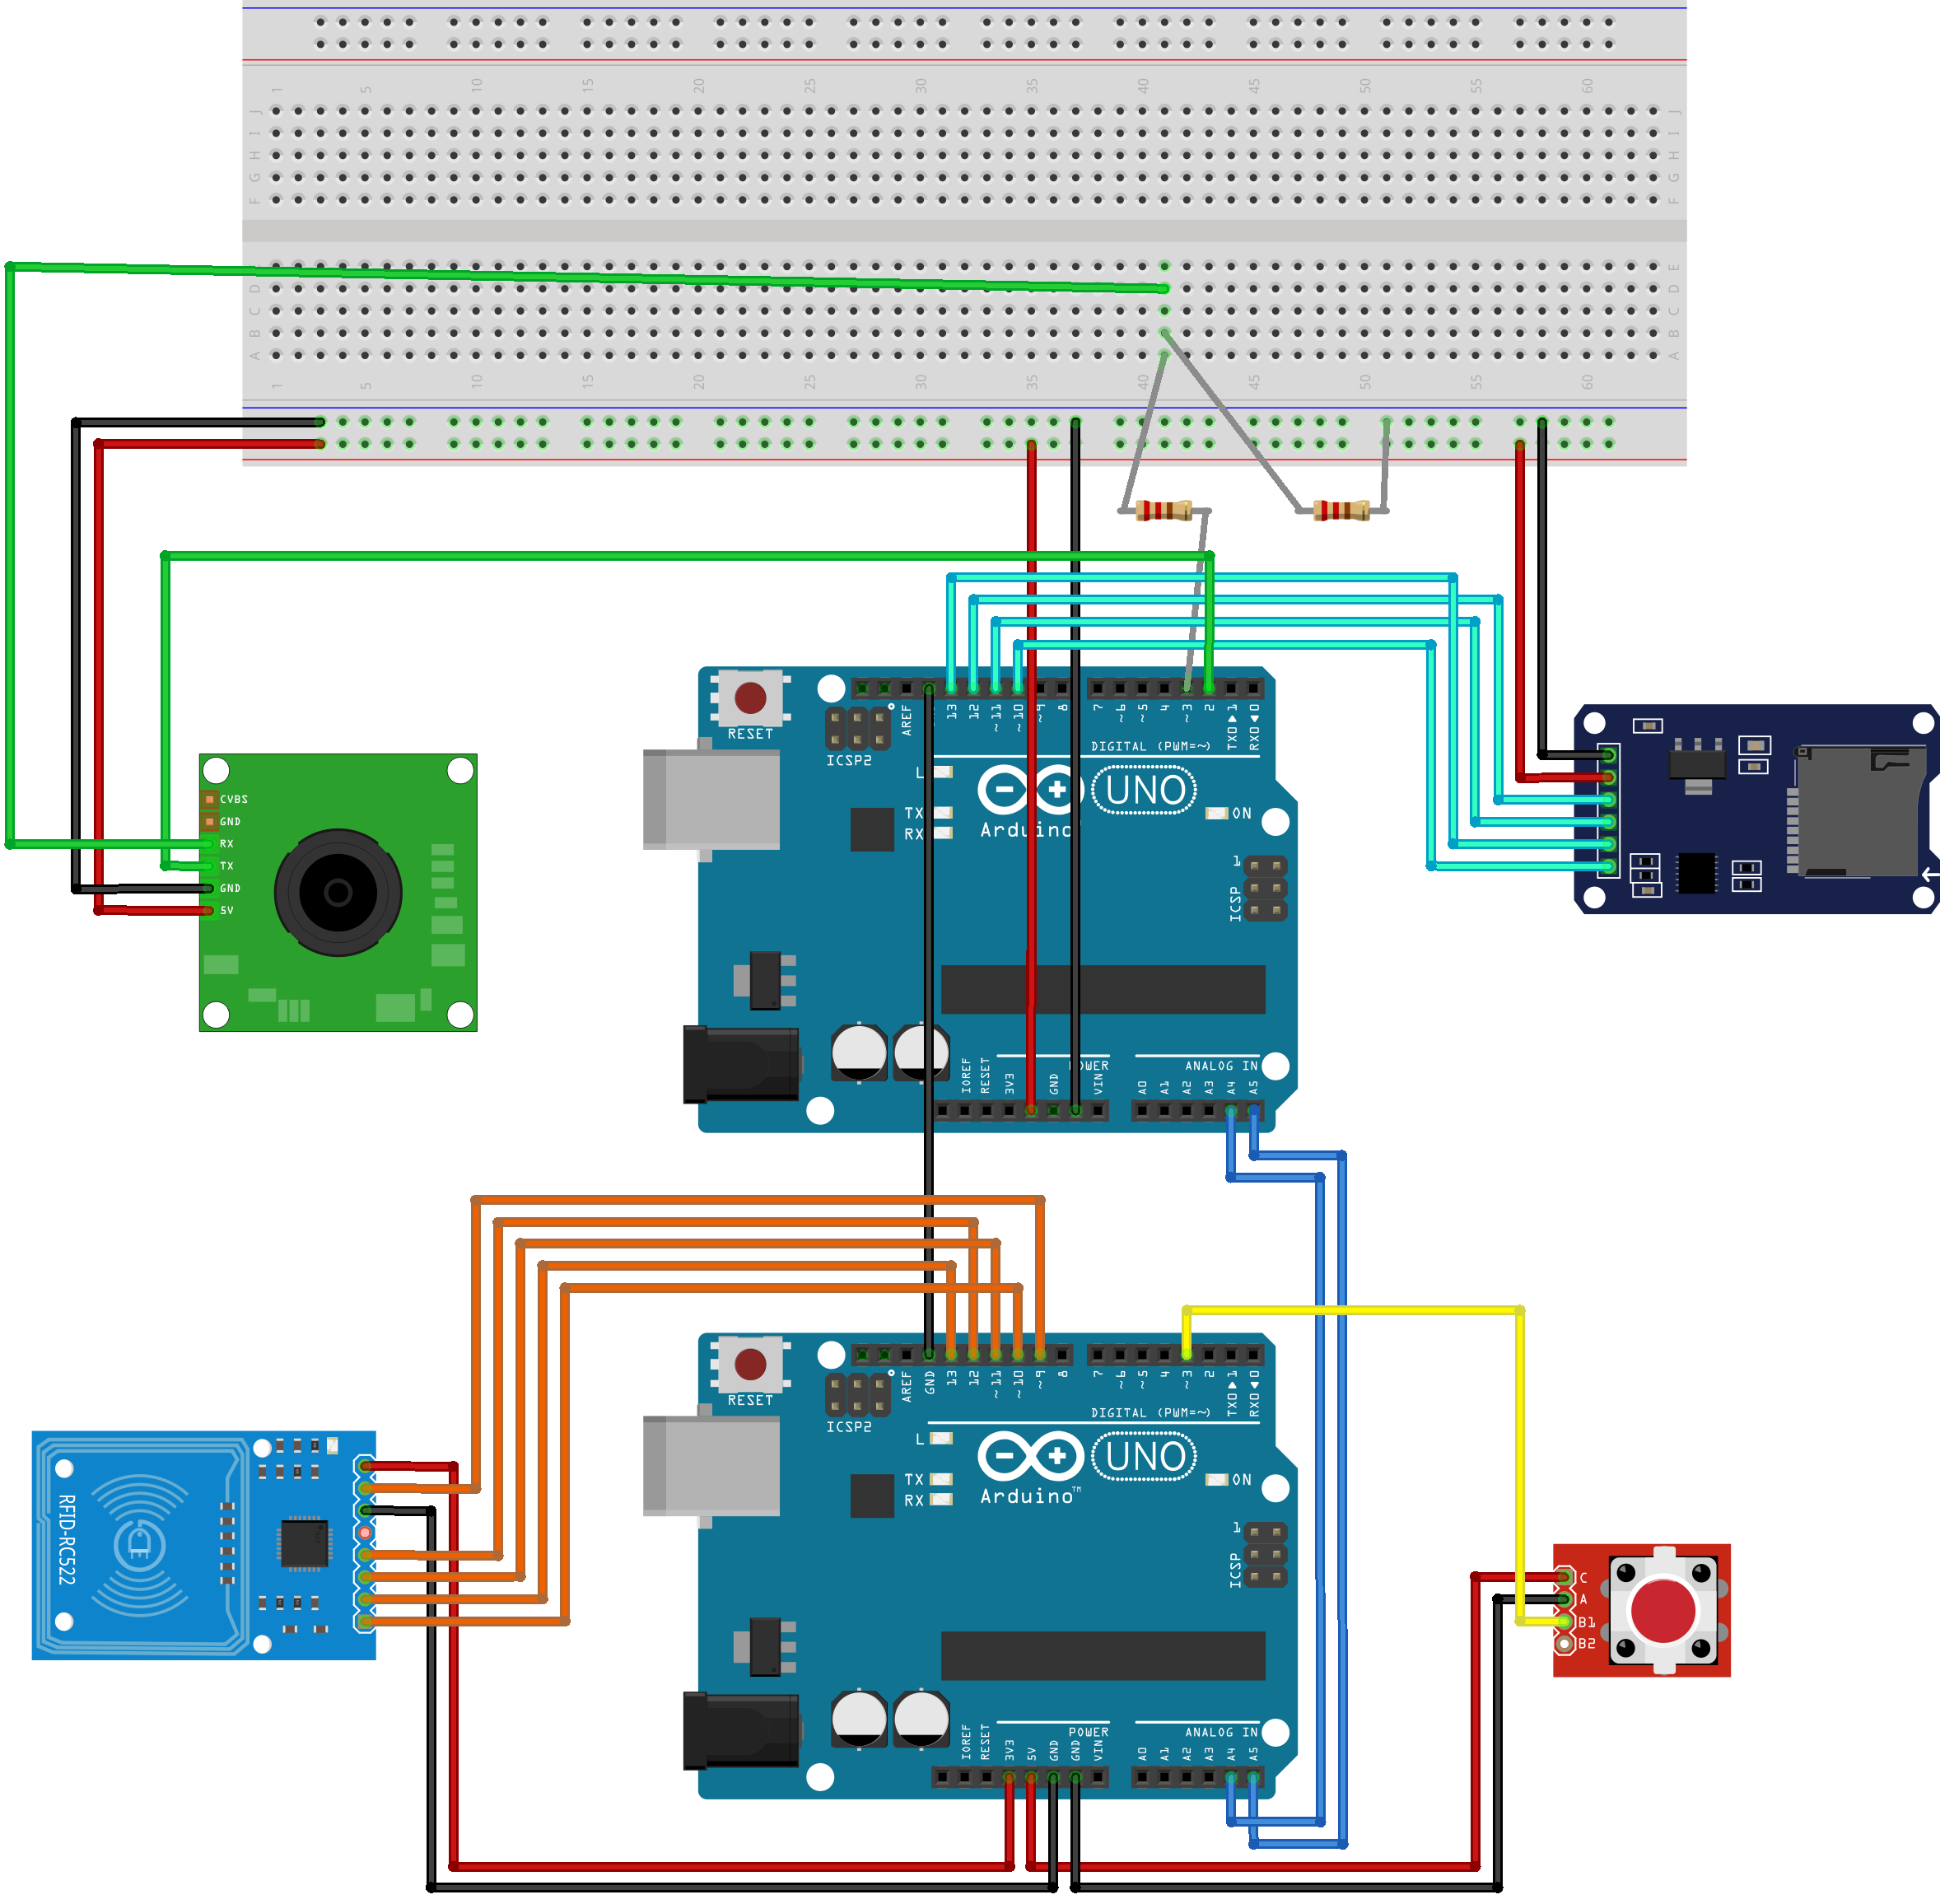
\includegraphics[width=1\textwidth]{uebersicht.png}}
    \caption{Verbindung der Komponenten in Steckplattenansicht\label{fig:uebersicht}}
\centering
\end{figure}

\noindent Der Aufbau des Überwachungssystems lässt sich in zwei Teilsysteme eingliedern. Beide Teilsysteme bestehen, wie in Abbildung \ref{fig:uebersicht} zu erkennen ist, aus jeweils einem \textit{Arduino Uno} und zwei weiteren Komponenten. 

Als erstes Teilsystem kann das in der Abbildung untere System betrachtet werden. Die verbundenen Komponenten sind der Button und das RFID-Modul.
Das zweite Teilsystem beinhaltet die Komponenten Kamera und SD-Karten-Modul. Aus der Abbildung ist zu erkennen, dass zwischen dem \texttt{RX}-Pin der Kamera und dem Arduino zwei \textit{Resistoren} geschaltet sind.

Die Kommunikation zwischen beiden Teilsystemen läuft über zwei Verbindungen von analogen Arduino-Pins. Die Entscheidung das Sicherheitssystem in zwei Bereiche zu teilen, bezieht sich daraus, dass die Kommunikation zwischen Arduinogeräten ebenfalls als spannendes Themenfeld der hardwarenahen Systemprogrammierung gesehen werden kann und von uns näher betrachtet werden wollte.
Die Schnittstellenanbindungen der Komponenten sind aus der unteren Tabelle auszulesen.


\begin{table}[htb]
\begin{tabular}{@{}lllll@{}}
\toprule
\multicolumn{2}{c}{Arduino 1} &  & \multicolumn{2}{c}{Arduino 2}                    \\ \cmidrule(r){1-2} \cmidrule(l){4-5} 
RFID\_SDA    & arduino\_d10   &  & CAMERA\_TX  & arduino\_d2                        \\
RFID\_SCK    & arduino\_d13   &  & CAMERA\_RX  & resistor $\rightarrow$ GND         \\
RFID\_MOSI   & arduino\_d11   &  &             & resistor $\rightarrow$ arduino\_d3 \\
RFID\_MISO   & arduino\_d12   &  & CAMERA\_GND & GND                                \\
RFID\_IRQ    & not connected  &  & CAMERA\_VCC & 5V                                 \\
RFID\_RST    & arduino\_d9    &  &             &                                    \\ 
RFID\_GND    & GND            &  & SD\_CS      & arduino\_d10                       \\
RFID\_VCC    & 3.3V           &  & SD\_SCK     & arduino\_d13                       \\
                &                &  & SD\_MOSI    & arduino\_d11                       \\
BTN\_S       & arduino\_d3    &  & SD\_MISO    & arduino\_d12                       \\
BTN\_-       & GND            &  & SD\_GND     & GND                                \\
BTN\_+       & 5V             &  & SD\_VCC     & 5V                                 \\ \bottomrule
\end{tabular}
\end{table}


\section{Funktionsablauf}
Der Funktionsablauf des Sicherheitssystems wurde im Sequenzdiagramm in Abbildung \ref{fig:sequenz} dargestellt.

Ein Protokollierungsauftrag startet mit dem Öffnen der Kühlschranktür, was durch das Drücken des Buttons simuliert wird. Hiernach überprüft das RFID-Modul ob ein Nutzer durch das Aufliegen eines RFID-Tokens erkannt werden kann. Wird ein Token erkannt, wird zusätzlich kontrolliert, ob diesem Nutzer der Zugriff zum Kühlschrank gestattet ist. Anhand dieser Informationen wird nun ein \texttt{Request-String} gebildet und an den zweiten Arduino übertragen. Dieser String beinhaltet mehrere Informationen:
%\pagebreak
\begin{enumerate}
\item Wurde ein Nutzer-Token benutzt?
\item Ist der Nutzer berechtigt den Kühlschrank zu benutzen?
\item Nutzer-ID
\end{enumerate}

\noindent Das Eintreffen des \texttt{Request-String} löst beim zweiten Arduino ein \textit{Event} aus. Dadurch schießt die Kamera einen Schnappschuss und speichert dieses Foto auf der SD-Karte. Zusätzlich wird in einem Text-Log hinterlegt welcher \texttt{Request-String} welche Foto-Datei produziert hat. Dies beendet einen Protokollierungsauftrag. Das Analysieren der Kühlschranknutzung kann folglich durch die Betrachtung der Logs und den Vergleich mit dem Bildmaterial durchgeführt werden. 

\begin{figure}[htb]
\centering
    {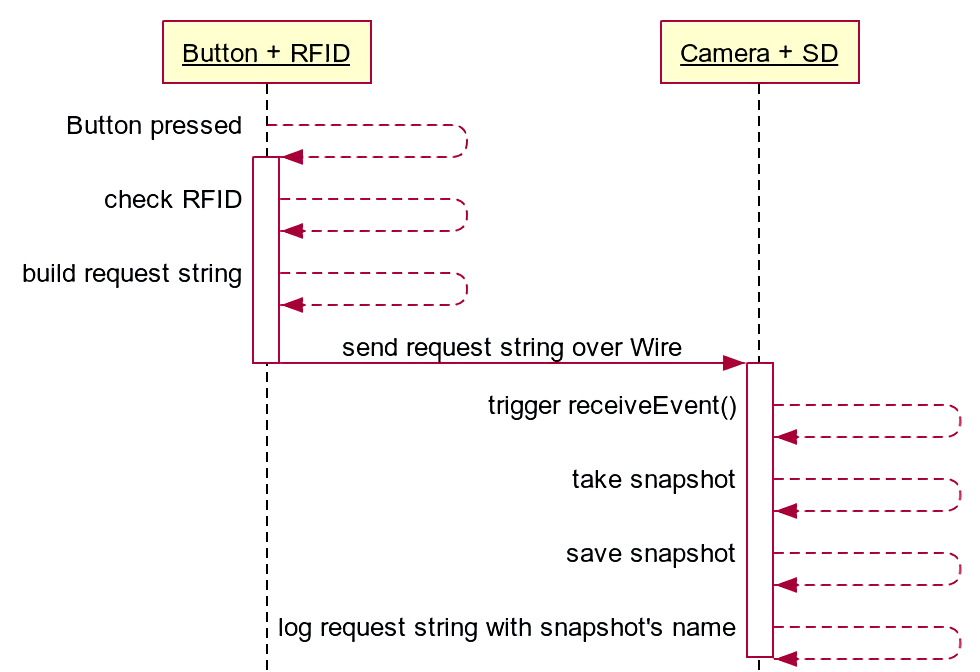
\includegraphics[width=.9\textwidth]{sequenz1.png}}
    \caption{Funktionsablauf anhand eines Sequenzdiagramms\label{fig:sequenz}}
\centering
\end{figure}


\section{Eigene Library zur Funkkommunikation}



\section{Repository}
\url{https://github.com/LeonardKoll/arduinofridge}

\end{document}